\section{Irregular designs and hierarchical extensions}
\label{sec:extensions}

The ordered-partition recursions remain valid when prior factors or multiple-sequence likelihoods can be expressed segment by segment. This section gives the corresponding models for irregular coordinates, shared changepoints, observed groups, and latent groups.

\subsection{Irregular designs: segment cohesion and boundary hazard}
Irregular coordinates can enter the partition prior in two statistically distinct ways. A complete-segment cohesion $c_u(i,j)$ assigns prior mass according to the physical span of $(i,j]$; an interior-boundary hazard $h_u(j)$ assigns prior mass to a candidate split at $u_j$. They can appear together in Equation~\eqref{eq:partition-prior}, but one does not imply the other.

\begin{figure}[!htbp]
  \centering
  \resizebox{0.96\columnwidth}{!}{
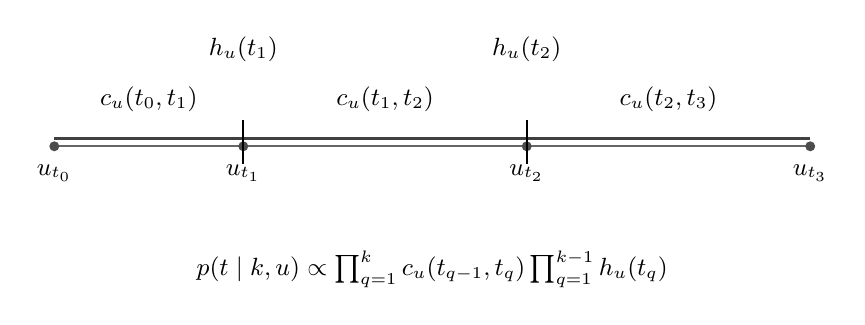
\begin{tikzpicture}[x=1.2cm,y=1cm]
\draw[line width=0.65pt,black!60] (0,0)--(8,0);
\foreach \x/\lab in {0/$u_{t_0}$,2/$u_{t_1}$,5/$u_{t_2}$,8/$u_{t_3}$}{
  \fill[black!70] (\x,0) circle (1.8pt);
  \node[below=3pt,font=\small] at (\x,0) {\lab};
}
\foreach \start/\finish/\text in {0/2/{c_u(t_0,t_1)},2/5/{c_u(t_1,t_2)},5/8/{c_u(t_2,t_3)}}{
  \draw[line width=1.15pt,black!75] (\start,0.1)--(\finish,0.1);
  \node[above=9pt,font=\small] at ({(\start+\finish)/2},0) {$\text$};
}
\draw[line width=0.85pt,black] (2,-.22)--(2,.34);
\draw[line width=0.85pt,black] (5,-.22)--(5,.34);
\node[above=27pt,font=\small] at (2,0) {$h_u(t_1)$};
\node[above=27pt,font=\small] at (5,0) {$h_u(t_2)$};
\node[font=\small,align=center,below=12mm] at (4,0) {$p(t\mid k,u)\propto\prod_{q=1}^{k}c_u(t_{q-1},t_q)\prod_{q=1}^{k-1}h_u(t_q)$};
\end{tikzpicture}
}
  \caption{Design-dependent partition prior. Segment cohesion and interior-boundary hazard represent different prior assumptions. The terminal endpoint receives no boundary-hazard factor.}
  \label{fig:cohesion-hazard-paper}
\end{figure}

\begin{theorem}[Local prior factors preserve exact inference]
\label{thm:local-prior-paper}
Replacing $A^{(r)}_{ij}$ by
$\widetilde A^{(r)}_{ij}=A^{(r)}_{ij}c_u(i,j)h_u(j)^{\1\{j<n\}}$
causes the sum-product recursion to enumerate exactly the unnormalized joint weights in Equation~\eqref{eq:partition-prior}. Dividing the terminal partition sum by $C_k(u)$ yields the proper fixed-$k$ marginal likelihood.
\end{theorem}
\begin{proof}
\textbf{Step 1 (factor the intended partition weight).}
For fixed $k$ and $t=(t_0,\ldots,t_k)$, multiply its independent segment marginal likelihoods by the conditional prior in Equation~\eqref{eq:partition-prior}.
\textbf{Step 2 (push each factor into a segment).}
Every segment ending at $t_q<n$ contributes the prior factor $c_u(t_{q-1},t_q)h_u(t_q)$, while the terminal segment ending at $n$ contributes only $c_u(t_{k-1},n)$. Thus $\prod_q\widetilde A^{(0)}_{t_{q-1},t_q}$ is exactly the likelihood product times the \emph{unnormalized} prior factor.
\textbf{Step 3 (sum over all partitions).}
Theorem~\ref{thm:sum-product} enumerates these path products once each, so $L_{k,n}$ is their unnormalized sum. Running the same recurrence with $A^{(0)}_{ij}=1$ enumerates exactly the prior weights and returns $C_k(u)$.
\textbf{Step 4 (normalize once, not once per block).}
Multiplication by $C_k(u)^{-1}$ in the fixed-count prior is common across partitions; hence $p(y\mid k)=L_{k,n}/C_k(u)$. Applying the same factor inside each block instead would produce an incorrect power of the prior normalizer.
\end{proof}

A boundary-process interpretation applies only to the hazard factor. Let
$\Lambda_j=\int_{u_{j-1}}^{u_j}\lambda(v)\dd v$ for an inhomogeneous Poisson process. Interval
occupancies are independent Bernoulli variables with probability $1-e^{-\Lambda_j}$. Conditional
on exactly $m$ occupied candidate intervals, the subset probability is proportional to the product
of Bernoulli odds, so the compatible local factor is
\begin{equation}
 h_u(j)\propto \frac{1-e^{-\Lambda_j}}{e^{-\Lambda_j}}=e^{\Lambda_j}-1.
\label{eq:poisson-hazard}
\end{equation}
Constant intensity and equal-width intervals recover an index-uniform fixed-count boundary prior when $c_u\equiv1$. Without conditioning on the number of occupied intervals, both occupied and unoccupied Bernoulli factors are part of the prior. Equation~\eqref{eq:poisson-hazard} does not justify multiplying a segment likelihood by its physical length; a duration-dependent cohesion is a separate prior choice.

\subsection{Renewal interpretation and refinement of an irregular design}
\label{sec:design-refinement}
The local prior factorization admits a renewal interpretation, but its conditioning matters. A conditional prior on partitions given a separately sampled count $k$ does not automatically induce a prior on the count.

\begin{proposition}[Renewal-length equivalence conditional on $k$]
\label{prop:renewal-equivalence-paper}
On an index grid with $0=t_0<t_1<\cdots<t_k=n$, let the positive segment lengths $d_q=t_q-t_{q-1}$ have an unnormalized renewal mass $g(d_q)\ge0$. Conditional on $\sum_qd_q=n$ and a fixed count $k$, the boundary distribution is
\[
p(t\mid k)=\frac{1}{C_k}\prod_{q=1}^{k}g(t_q-t_{q-1}),\qquad
C_k=\sum_{t\in\mathcal T_k}\prod_{q=1}^{k}g(t_q-t_{q-1}).
\]
For geometric $g(d)=\rho(1-\rho)^{d-1}$, $0<\rho<1$, the product is constant over $\mathcal T_k$, and thus $p(t\mid k)$ is uniform regardless of $\rho$.
\end{proposition}
\begin{proof}
\textbf{Step 1 (one-to-one correspondence).} Each ordered partition uniquely determines a composition $(d_1,\ldots,d_k)$ of $n$ into positive integers, and conversely the partial sums of each such composition recover the boundaries.
\textbf{Step 2 (condition the renewal mass).} The unnormalized composition weight is $\prod_qg(d_q)$. Summing those weights over every admissible composition defines $C_k$, so normalizing yields the displayed conditional distribution.
\textbf{Step 3 (geometric specialization).} For $g(d)=\rho(1-\rho)^{d-1}$, the product equals $\rho^k(1-\rho)^{\sum_qd_q-k}=\rho^k(1-\rho)^{n-k}$, independent of $t$ at fixed $k$. The factor cancels against $C_k$ and cannot push the separately specified segment-count prior $p(k)$ toward one or toward $n$.
\end{proof}

\begin{proposition}[Score preservation under grid refinement]
\label{prop:refinement-paper}
Suppose a candidate-coordinate grid is refined by adding locations carrying no new observations. Embed an original partition into the refined grid by retaining all of its physical segment endpoints and placing no boundary at a newly inserted location. Each inherited block then has the same likelihood integral; any cohesion or hazard factor depending only on unchanged physical endpoints and retained boundary weights has the same unnormalized prior contribution. The fully normalized partition posterior need not remain unchanged if new boundary locations are made admissible.
\end{proposition}
\begin{proof}
\textbf{Step 1 (likelihood equality).} Each inherited refined block contains exactly the original observations and descriptors, so its likelihood product and prior-integrated segment likelihood agree with those of the original block.
\textbf{Step 2 (prior equality for inherited paths).} Preserving physical endpoints preserves a cohesion depending only on those endpoints; by hypothesis, each retained interior boundary also retains its hazard factor. Multiplying across blocks thus gives the same unnormalized path weight.
\textbf{Step 3 (why posterior equality fails).} Refinement that admits an additional cut creates extra partitions in the sum defining $C_k$ and in the data-dependent partition sum. Even if every inherited path has unchanged weight, the two new normalizers generally differ. The equality is for inherited path scores, not for the whole posterior.
\end{proof}

\paragraph{Physical interval conventions.}
Observation locations $x_1<\cdots<x_n$ and candidate boundary coordinates $u_0<\cdots<u_n$ are distinct objects. Interior cell edges may be set to $u_i=(x_i+x_{i+1})/2$ for $1\le i<n$ and endpoints determined from the scientific measurement domain. The complete-segment span $u_j-u_i$ is not the same object as the observation gap $x_{i+1}-x_i$. An inhomogeneous Poisson boundary process can supply hazard factors through integrated intensities, but an interval-length cohesion does not automatically produce that process.


\subsection{Shared changepoints across multiple sequences}
Suppose $S$ aligned sequences share a boundary vector while retaining sequence-specific segment parameters and priors. Conditional independence gives a pooled segment marginal likelihood.

\begin{figure}[!htbp]
  \centering
  \resizebox{0.96\columnwidth}{!}{\begin{tikzpicture}
\node[latent] (t) {$t$};
\node[latent,below=12mm of t] (theta) {$\theta^{(s)}_q$};
\node[obs,below=12mm of theta] (y) {$y^{(s)}_i$};
\node[const,right=11mm of y] (d) {$d^{(s)}_i$};
\edge {theta,d} {y}
\edge {t} {theta}
\plate {seg} {(theta)} {$q=1{:}k$}
\plate {subj} {(seg)(y)(d)} {$s=1{:}S$}
\node[secondarybox,text width=42mm,right=27mm of theta] (prod) {$\log A^{\rm pool}_{ij}=\sum_s\log A^{(s)}_{ij}$};
\draw[arrSecondary] (subj.east)--(prod.west);
\end{tikzpicture}
}
  \caption{Hierarchical common-changepoint model with sequence-specific segment parameters. Conditional independence makes the sequence-specific segment marginal likelihoods multiply.}
  \label{fig:shared-boundary-paper}
\end{figure}

\begin{assumption}[Common candidate set]
\label{ass:shared-support}
The sequences are aligned to a common ordered candidate set. Every candidate partition considered by the common-changepoint model is admissible for every sequence after the declared missing-data or exposure convention. Conditional on the common partition, sequences and their segment parameters are independent, and all sequence-specific segment marginal likelihoods are finite and positive on the common support.
\end{assumption}

\begin{theorem}[Exact pooling under a common partition]
\label{thm:pooling-paper}
Under Assumption~\ref{ass:shared-support}, the pooled segment marginal likelihood is
\begin{equation}
 A^{(0),\mathrm{pool}}_{ij}=\prod_{s=1}^{S}A^{(0,s)}_{ij},
 \qquad
 \ell^{\mathrm{pool}}_{ij}=\sum_{s=1}^{S}\ell^{(s)}_{ij}.
\label{eq:pooling}
\end{equation}
Using this array in Section~\ref{sec:exact-inference} gives the exact posterior distribution over the common partition. Conditional sequence-specific parameter posteriors are recovered from the original sequence-specific conjugate updates.
\end{theorem}
\begin{proof}
\textbf{Step 1 (integrate independently within a segment).}
For sequence $s$, write $\theta_{B,s}$ for its parameter on a candidate shared segment $B=(i,j]$. By the independent segment priors, integrating its observations over $\theta_{B,s}$ yields $A^{(0,s)}_{ij}$.
\textbf{Step 2 (factor across sequences).}
The model assumes conditional independence across sequences given the shared partition, and the subject-specific segment parameters are independent a priori. Tonelli's theorem for nonnegative integrands permits exchanging product and integration, so
\[
\int\prod_{s=1}^{S}p(y_B^{(s)}\mid\theta_{B,s})p_s(\theta_{B,s})\,\dd\theta_{B,1:S}
=\prod_{s=1}^{S}A^{(0,s)}_{ij}.
\]
Taking logarithms gives the additive log-score formula in Equation~\eqref{eq:pooling}.
\textbf{Step 3 (apply the unchanged partition recursion).}
Multiplication over segments produces the exact integrated joint likelihood conditional on every shared partition. Applying the same partition prior and the sum-product recursion therefore yields its exact boundary and count posterior. Given a partition, conjugate posterior calculations for each sequence's segment parameters remain separate; they are not automatically a single joint conjugate density integrated over all partitions.
\end{proof}

Known groups are handled by applying Equation~\eqref{eq:pooling} separately within each observed group. The following asymptotic statement is restricted to a finite candidate set and requires information to accumulate across sequences.

\begin{theorem}[Finite-candidate consistency for a common partition]
\label{thm:shared-consistency-paper}
Let $\mathcal T$ be finite and contain a data-generating candidate $t^\star$. For sequence $s$, let $M_s(t)>0$ be the integrated score used by the common-partition model. Assume independent sequences, $p(t^\star)>0$, and for each $t\ne t^\star$:
\begin{enumerate}
\item $\mathbb E|\log M_s(t^\star)-\log M_s(t)|<\infty$;
\item a strong law holds for the centered log-score differences; and
\item $\liminf_{S\to\infty}S^{-1}\sum_{s=1}^{S}\mathbb E[\log M_s(t^\star)-\log M_s(t)]=\delta_t>0$.
\end{enumerate}
Then $p(t^\star\mid y^{(1:S)})\to1$ almost surely, and every joint MAP segmentation is eventually $t^\star$ almost surely.
\end{theorem}
\begin{proof}
\textbf{Step 1 (posterior ratio for an incorrect candidate).}
Fix $t\ne t^\star$ and put $D_s(t)=\log M_s(t^\star)-\log M_s(t)$. Bayes' rule gives
\[
\frac{p(t\mid y^{(1:S)})}{p(t^\star\mid y^{(1:S)})}
=\frac{p(t)}{p(t^\star)}\exp\!\left\{-\sum_{s=1}^{S}D_s(t)\right\}.
\]
If $p(t)=0$, the ratio is identically zero and needs no further argument.
\textbf{Step 2 (accumulation of log-score separation).}
The assumed strong law makes $S^{-1}\sum_s[D_s(t)-\mathbb ED_s(t)]\to0$ almost surely. The strictly positive limiting lower bound on the mean expected difference then gives $\liminf_{S\to\infty}S^{-1}\sum_sD_s(t)\ge\delta_t>0$ almost surely.
\textbf{Step 3 (vanishing posterior odds).}
The exponential factor in Step~1 tends to zero at an exponential rate in $S$, and the fixed prior odds cannot prevent this. Hence every incorrect candidate has posterior mass asymptotically negligible relative to $t^\star$.
\textbf{Step 4 (finite candidate set).}
There are only finitely many $t\in\mathcal T$, so the sum of incorrect posterior ratios tends to zero. Normalization yields $p(t^\star\mid y^{(1:S)})\to1$, and eventually its posterior mass exceeds that of every incorrect $t$, proving the joint MAP conclusion. The theorem requires an informative average across growing numbers of sequences; adding one informative sequence and arbitrarily many uninformative ones does not satisfy the positive-gap condition.
\end{proof}

One fixed informative sequence is insufficient for this theorem because its contribution vanishes in the average as $S$ increases. The assumption requires an accumulating average expected log-score gap.

\subsection{Finite latent-group template model}
For sequence $s$ and deterministic segmentation template $\tau=(k,t)$, consider the score
\begin{equation}
 S_s(\tau)=\frac{p(k)}{C_k}\prod_{q=1}^{k}
 A^{(0,s)}_{t_{q-1},t_q}\gamma_u(t_{q-1},t_q).
\label{eq:sequence-template-score-paper}
\end{equation}
These subject-template scores are not required to integrate to one over the data space. We therefore define the finite criterion
\begin{align}
\mathcal F(\pi,\tau)
&=\sum_{s=1}^{S}\log\!\left\{\sum_{g=1}^{G}\pi_gS_s(\tau_g)\right\},\nonumber\\
&\hspace{8mm}\pi_g\ge0,\qquad \sum_g\pi_g=1.
\label{eq:latent-group-objective}
\end{align}
This is a latent-group clustering criterion. It is not interpreted as a finite-mixture likelihood unless each $S_s(\tau_g)$ is a normalized sampling density.



For row-stochastic auxiliary weights $r_{sg}$, Jensen's inequality gives
\begin{align}
\mathcal F(\pi,\tau)&\ge\mathcal Q(r,\pi,\tau),\nonumber\\
\mathcal Q(r,\pi,\tau)
&=\sum_{s,g}r_{sg}\bigl[\log\pi_g+\log S_s(\tau_g)-\log r_{sg}\bigr],
\label{eq:latent-group-bound}
\end{align}
with equality at
\begin{equation}
 r_{sg}=\frac{\pi_gS_s(\tau_g)}{\sum_h\pi_hS_s(\tau_h)}.
\label{eq:auxiliary-weights}
\end{equation}
The mixing-weight update is $\pi_g=S^{-1}\sum_s r_{sg}$. Let $n_g=\sum_s r_{sg}$. For a candidate segment count $k$, substitution of Equation~\eqref{eq:sequence-template-score-paper} into the minorizer gives the count offset $n_g\{\log p(k)-\log C_k\}$ and the max-sum local score
\begin{equation}
\ell^{(g)}_{ij}=\sum_{s=1}^{S}r_{sg}\log A^{(0,s)}_{ij}
                  +n_g\log\gamma_u(i,j).
\label{eq:template-local-score}
\end{equation}
The template update solves the fixed-$k$ max-sum problem and then compares the offset-adjusted terminal values across the allowed segment counts.

\begin{theorem}[Monotonicity of exact latent-group updates]
\label{thm:template-monotonicity-paper}
An iteration that sets $r$ by Equation~\eqref{eq:auxiliary-weights}, maximizes $\mathcal Q$ over $\pi$, and exactly maximizes every responsibility-weighted template criterion using Equation~\eqref{eq:template-local-score} and its segment-count offset over the declared finite candidate set cannot decrease $\mathcal F$.
\end{theorem}
\begin{proof}
\textbf{Step 1 (construct a tight Jensen minorizer).}
For any row-stochastic $r$, Jensen's inequality applied to the positive sum over group templates gives $\mathcal F(\pi,\tau)\ge\mathcal Q(r,\pi,\tau)$. Choosing $r$ as in Equation~\eqref{eq:auxiliary-weights} at the current $(\pi^{\rm old},\tau^{\rm old})$ makes the inequality an equality.
\textbf{Step 2 (update group weights).}
At fixed $r$ and templates, the $\pi$-dependent terms are $\sum_gn_g\log\pi_g$. Maximization on the probability simplex gives $\pi_g=n_g/S$ for positive group masses, under the declared boundary convention for empty groups. This cannot decrease $\mathcal Q$.
\textbf{Step 3 (update templates exactly).}
For group $g$, substitute the score definition in Equation~\eqref{eq:sequence-template-score-paper} into $\sum_sr_{sg}\log S_s(\tau_g)$. Every segment receives $\sum_sr_{sg}\log A^{(0,s)}_{ij}+n_g\log\gamma_u(i,j)$, and the count offset is $n_g[\log p(k)-\log C_k]$. Max-sum dynamic programming and comparison across all admissible $k$ globally maximize this coordinate of the minorizer.
\textbf{Step 4 (chain the inequalities).}
Let $(\pi^{\rm new},\tau^{\rm new})$ denote the updated parameters. Then
\[
\mathcal F(\pi^{\rm new},\tau^{\rm new})
\ge\mathcal Q(r,\pi^{\rm new},\tau^{\rm new})
\ge\mathcal Q(r,\pi^{\rm old},\tau^{\rm old})
=\mathcal F(\pi^{\rm old},\tau^{\rm old}).
\]
The argument establishes monotonicity of the stated finite \emph{score-clustering} criterion, not maximization of a normalized generative mixture likelihood or global convergence across restarts.
\end{proof}


\begin{proposition}[Permutation symmetry of the finite template criterion]
\label{prop:label-symmetry-paper}
For every permutation $\sigma$ of the $G$ group indices, simultaneously replacing $(\pi_g,\tau_g)$ by $(\pi_{\sigma(g)},\tau_{\sigma(g)})$ leaves $\mathcal F$ unchanged. Consequently, the numerical labels of fitted templates are not identified by this criterion; distinct groups with identical templates can also produce non-uniqueness beyond label permutations.
\end{proposition}
\begin{proof}
\textbf{Step 1 (permute inside each sequence score).}
For subject $s$, relabeling the terms of the finite sum gives $\sum_g\pi_{\sigma(g)}S_s(\tau_{\sigma(g)})=\sum_g\pi_gS_s(\tau_g)$, because $\sigma$ is a bijection.
\textbf{Step 2 (preserve the objective).}
Taking the logarithm and summing the unchanged subject terms leaves Equation~\eqref{eq:latent-group-objective} invariant.
\textbf{Step 3 (non-uniqueness).}
If a maximizing set of templates is relabeled, it remains maximizing. If two templates coincide, their contributions can also be aggregated with changed mixture weights without changing their combined term, giving an additional source of non-identifiability. A plotting convention may canonically order labels, but it does not establish parameter identifiability or optimality across restarts.
\end{proof}

Template-label permutations, coincident templates, and an oversized $G$ can make the optimum non-unique. No finite-mixture identifiability or generative-model consistency claim is made. Multiple initializations must be compared using the criterion evaluated at their \emph{final} iterates, rather than a value recorded before the last update.
